\section{Modeling Sequential Data}
Recurrent Neural Networks (RNNs) are deep learning models that dont just take 
the data itself into account but also takes into account a temporal sequence
of data. This allows it to exhibit temporal dynamic behavior. It uses it's 
internal state to process variable length sequences of inputs. RNNs arised 
in the 80s and have proven themselves in applicable tasks such as handwriting
recognition, speech recognition, natural language processing, tim series 
forecasting and many others.

\section{LSTM}
the Long short-term memory networks were invented in 1997 and set accuracy
records in multiple domains. These networks have feedback connections.

\section{Computations}

\begin{figure}[H]
\centering
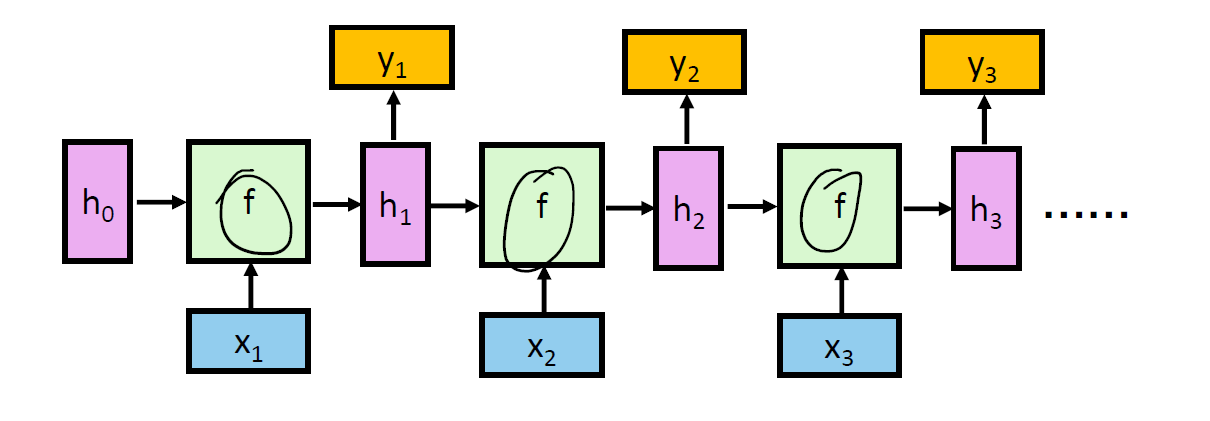
\includegraphics[scale=0.25]{figures/RNN.PNG}
\caption{Recurrent Neural Network architecture}
\end{figure}

The forward calculations in this layer is as follows

\begin{equation*}
    h_{l} = \phi(W^T h_{l-1} + U^T x_{l})
\end{equation*}

and you see that the calculations depend on all the following previous 
calculations as the feature $x$ at each timestep.

\section{Challenges with vanilla RNNs}
They are not able to capture long-term dependencies. It tends to forget old
information (markov assumption?). Also, when performing backpropagation they 
are prone to the exploding/vanishing gradients problem. Inference is also
slow.

